\documentclass{standalone}

\usepackage{xcolor}

\usepackage{fontspec}
\usepackage{pgfgantt}

\definecolor{darkgreen}{RGB}{100,200,100}

\begin{document}
  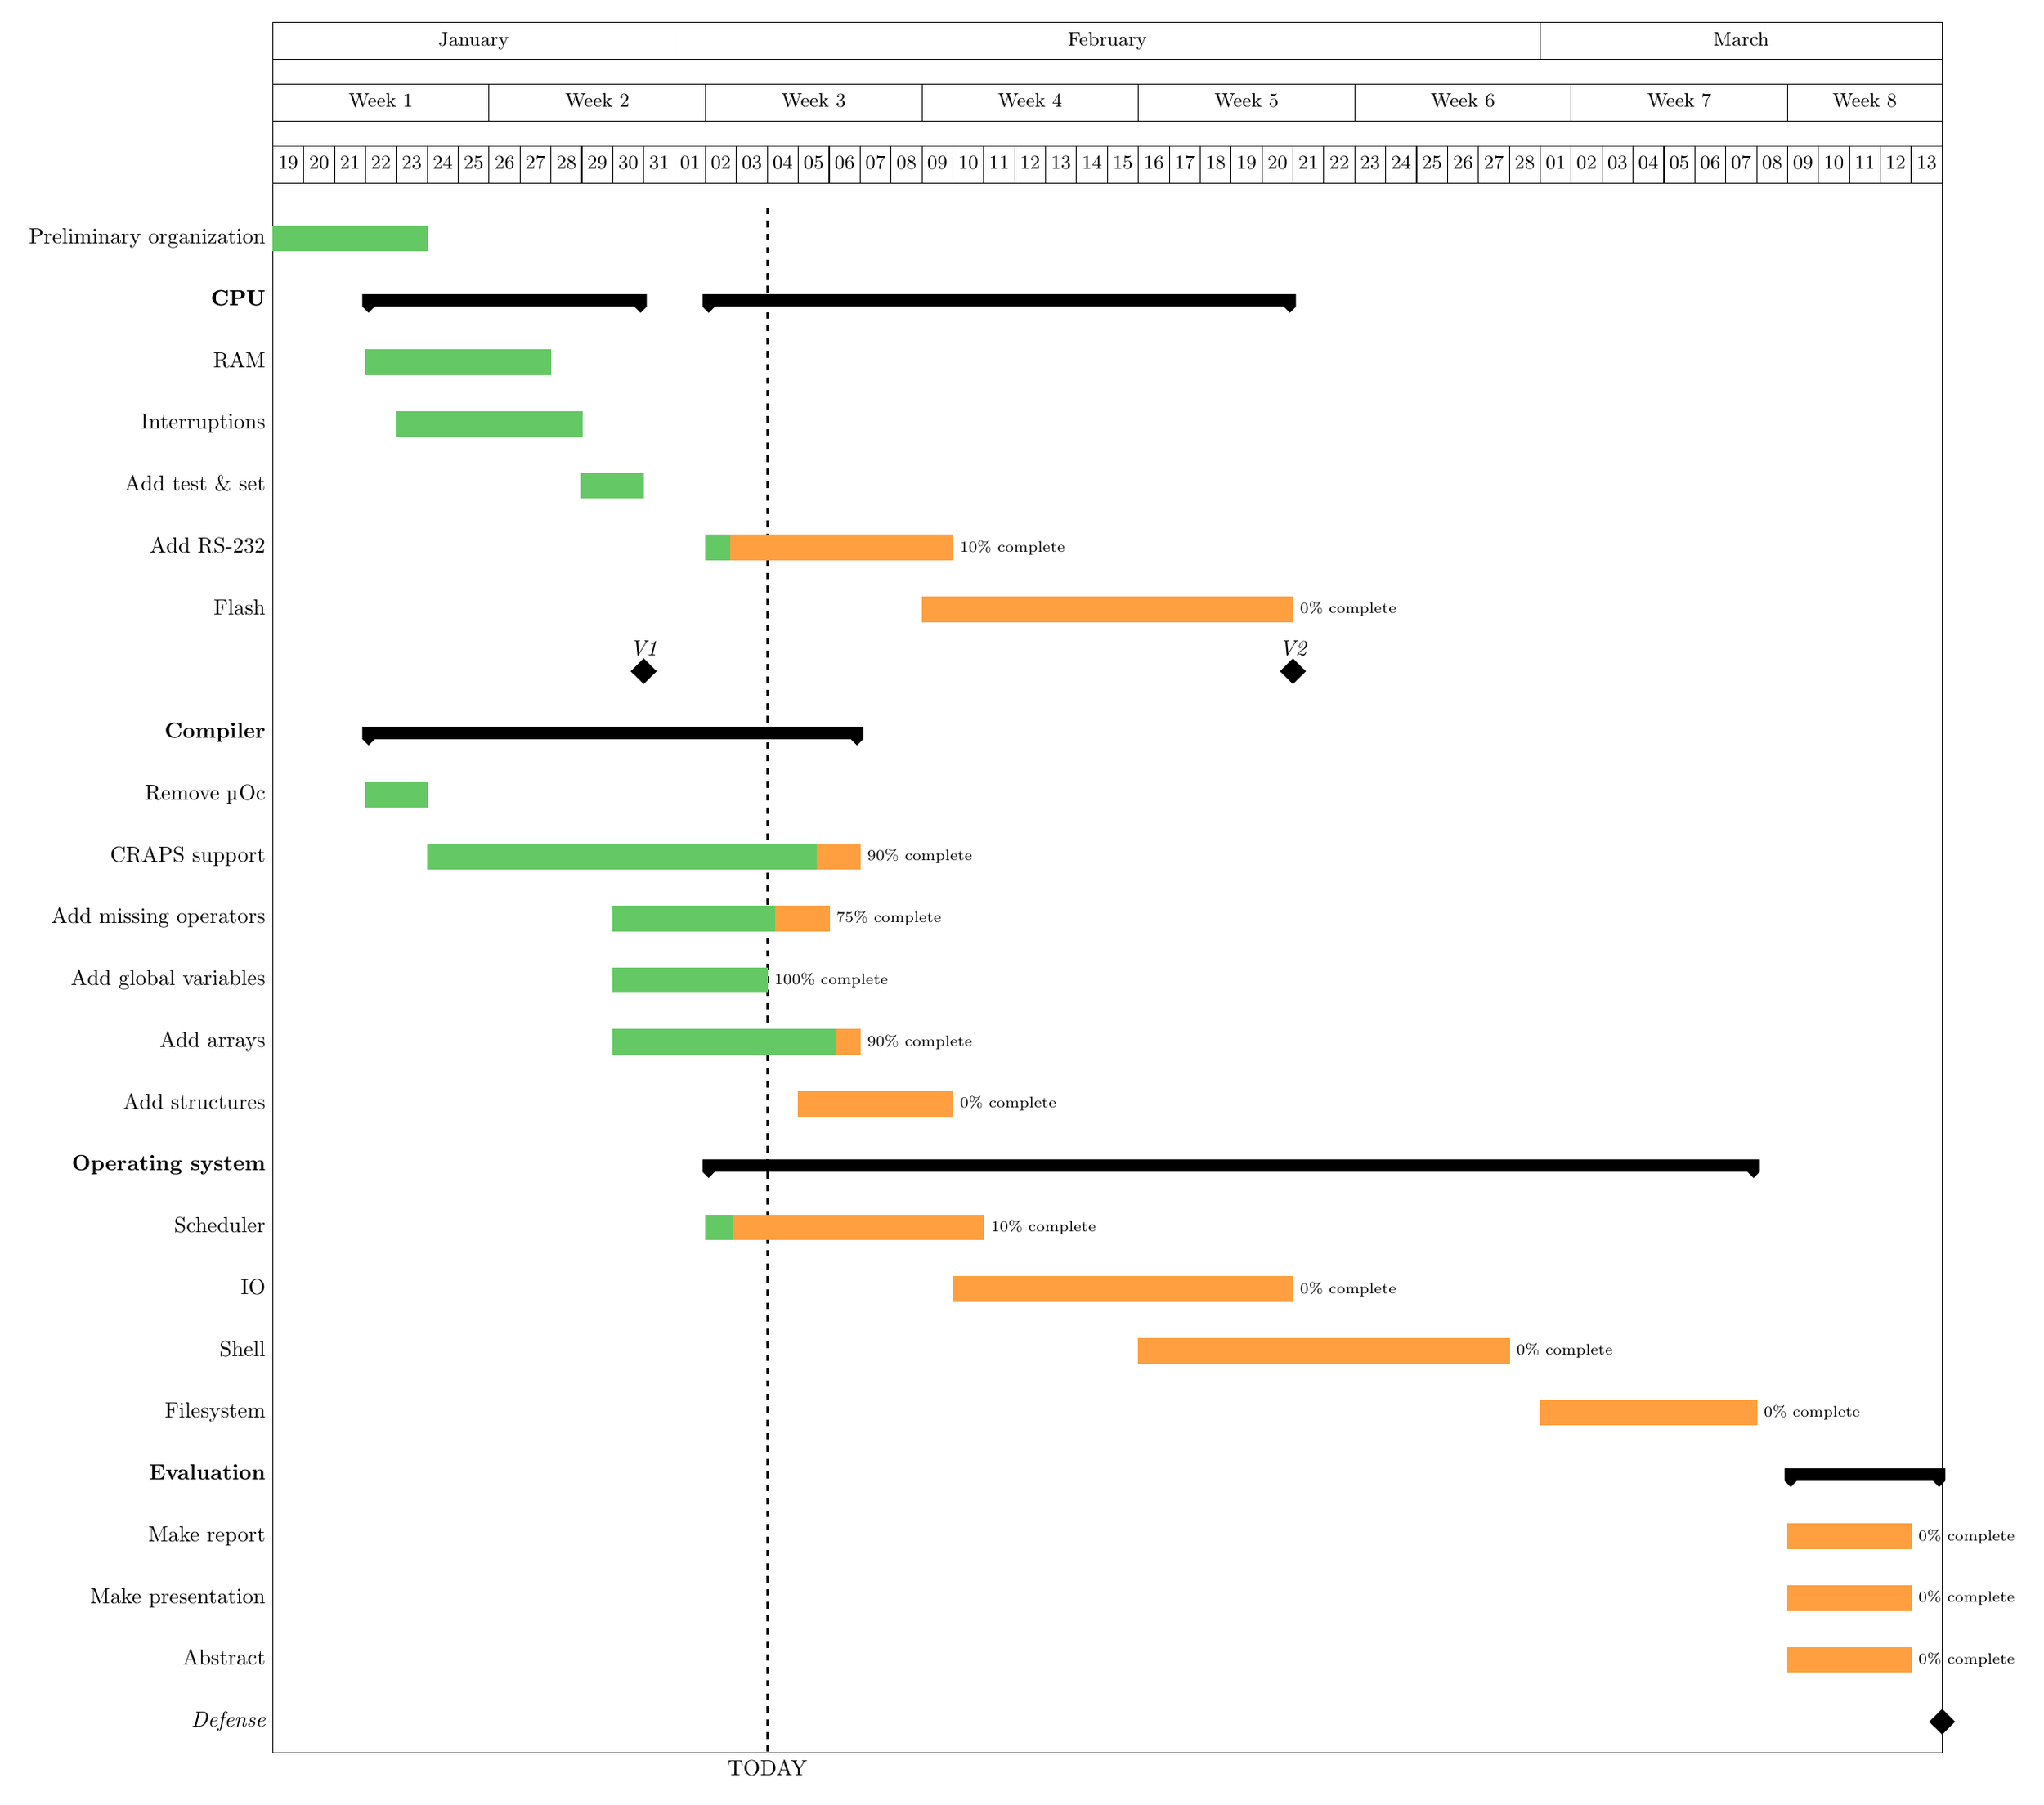
\begin{tikzpicture}
    \begin{ganttchart}[
        /pgf/outer xsep=+0pt,
        time slot format=isodate, /pgfgantt/time slot format/base century=20
        bar label font=\normalsize\color{black!50},
        bar/.append style={darkgreen},
        bar incomplete/.append style={orange!75},
        today=15-02-03
      ]{15-01-19}{15-03-13}
      \gantttitlecalendar{month=name, week, day}                              \\

      \ganttbar{Preliminary organization}{15-01-19}{15-01-23}                 \\

      \ganttgroup{CPU}{15-01-22}{15-01-30}
      \ganttgroup{CPU}{15-02-02}{15-02-20}                                    \\
          \ganttbar[name=RAM]{RAM}{15-01-22}{15-01-27}                        \\
          \ganttbar[name=IT]{Interruptions}{15-01-23}{15-01-28}               \\
          \ganttbar{Add test \& set}{15-01-29}{15-01-30}                      \\
          \ganttbar[progress=10]{Add RS-232}{15-02-02}{15-02-09}              \\

          \ganttbar[name=flash, progress=0]{Flash}{15-02-09}{15-02-20}        \\

          \ganttmilestone[inline]{V1}{15-01-30}
          \ganttmilestone[inline]{V2}{15-02-20}                               \\

      \ganttgroup[name=comp1]{Compiler}{15-01-22}{15-02-06}                   \\
          \ganttbar[name=MOC]{Remove µOc}{15-01-22}{15-01-23}                 \\
          \ganttbar[name=CRAPS, progress=90]{CRAPS support}{15-01-24}{15-02-06} \\
          \ganttbar[progress=75]{Add missing operators}{15-01-30}{15-02-05}   \\
          \ganttbar[progress=100]{Add global variables}{15-01-30}{15-02-03}   \\
          \ganttbar[progress=90]{Add arrays}{15-01-30}{15-02-06}              \\
          \ganttbar[progress=0]{Add structures}{15-02-05}{15-02-09}           \\

      \ganttgroup[name=os]{Operating system}{15-02-02}{15-03-07}              \\
          \ganttbar[progress=10]{Scheduler}{15-02-02}{15-02-10}               \\
          \ganttbar[progress=0]{IO}{15-02-10}{15-02-20}                       \\
          \ganttbar[progress=0]{Shell}{15-02-16}{15-02-27}                    \\
          \ganttbar[name=FS, progress=0]{Filesystem}{15-02-29}{15-03-07}      \\

      \ganttgroup[name=final]{Evaluation}{15-03-09}{15-03-13}                 \\
          \ganttbar[progress=0]{Make report}{15-03-09}{15-03-12}              \\
          \ganttbar[progress=0]{Make presentation}{15-03-09}{15-03-12}        \\
          \ganttbar[progress=0]{Abstract}{15-03-09}{15-03-12}                 \\
          \ganttmilestone{Defense}{15-03-13}

      %\ganttlink{flash}{FS}
    \end{ganttchart}
  \end{tikzpicture}
\end{document}
